Autoformer là 1 mô hình học sâu (Deep Learning) cải tiến kiến trúc phân rã từ mô hình Transformer truyền thống để phân tách dữ liệu chuỗi thời gian thành các thành phần (components) theo mùa (seasonality) và xu hướng (trend). Bao gồm kiến trúc phân rã sâu, cơ chế tự động tương quan (Autocorrelation), bộ mã hóa (Encoder) và bộ giải mã (Decoder) tương ứng.

\begin{figure}[htbp]
\centerline{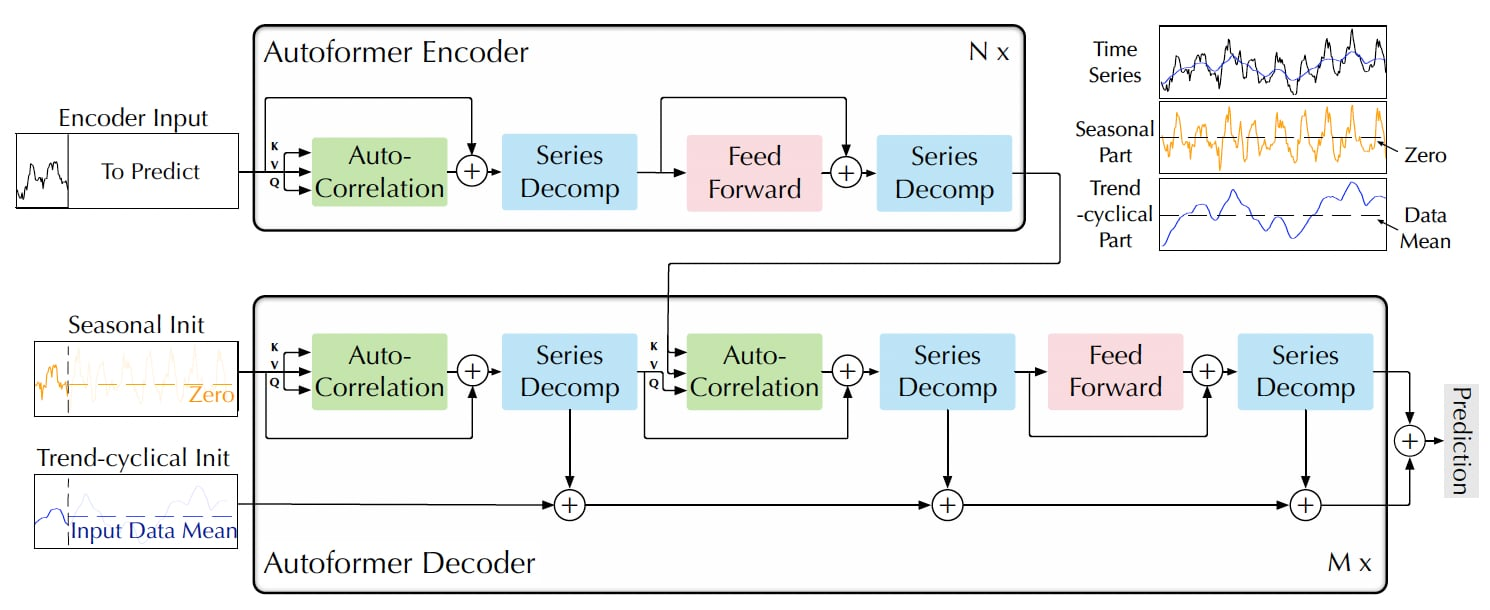
\includegraphics[width=0.4\textwidth]{img/autoformer.jpg}}
\caption{Tổng quan mô hình Autoformer.}
\label{fig}
\end{figure}

Decomposition Architecture – kiến trúc phân rã được xây dựng để nhằm nâng cao khả năng mô hình phân tách các thành phân trên chính xác hơn. Series decomposition block - khối phân tách dữ liệu dạng chuỗi, được sử dụng để trích xuất dần dần xu hướng ổn định dài hạn từ các biến ẩn trung gian được dự đoán. Cụ thể hơn, đó là thực hiện điều chỉnh đường trung bình động để làm dịu đi các biến động định kỳ và làm nổi bật các xu hướng dài hạn. Khối Encoder - bộ mã hóa, có nhiệm vụ tập trung vào việc mô hình hóa các thành phần có tính mùa vụ, đầu
ra của khối Encoder này chứa thông tin theo mùa trong quá khứ và sẽ được sử dụng làm thông tin chéo để giúp bộ giải mã tinh chỉnh kết quả dự đoán. Tiếp theo là đến khối Decoder - bộ giải mã, gồm 2 thành phần: cấu trúc tích lũy cho các thành phần theo chu kỳ xu hướng và cơ chế Tự tương quan (Autocorrelation) xếp chồng cho các thành phần theo mùa. \newline Như đã nói ở trên, Autoformer cũng giới thiệu 1 phương pháp tự động tương quan (Autocorrelation) cải tiến để thay thế cho self-attention trong mô hình Transformer chuẩn. Cơ chế tự động tương quan này phát hiện các phụ thuộc dựa trên thời gian bằng cách tính toán tự tương quan chuỗi và tổng hợp các chuỗi con tương tự bằng cách tổng hợp độ trễ thời gian, cho phép mô hình tận dụng sự phụ thuộc theo thời gian, từ đó cải thiện hiệu suất của mô hình tổng thể.

\begin{figure}[htbp]
\centerline{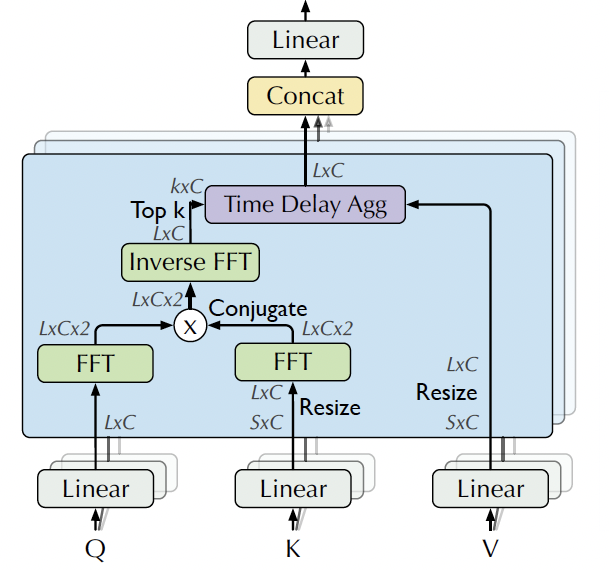
\includegraphics[width=0.4\textwidth]{img/autocorrelation.png}}
\caption{Cơ chế Auto-Correlation.}
\label{fig}
\end{figure}